\documentclass[10pt,a4paper]{article}
\usepackage[english]{babel}
\usepackage[utf8]{inputenc}
\usepackage[T1]{fontenc}
\usepackage{listings}
\usepackage{gensymb}
\usepackage[ddmmyy]{datetime}
\usepackage{graphicx}

%
% COMPILE USING PDFLATEX
%

\newcommand{\mnfysrppic}{\texttt{mn-fysrp-pic}}
\newcommand{\reffig}[1]{Fig.~\ref{fig:#1}}
\newcommand{\refapp}[1]{App.~\ref{app:#1}}
\newcommand{\refsec}[1]{Sec.~\ref{sec:#1}}
\renewcommand{\dateseparator}{.}
\def\labelitemi{\tiny$\bullet$}
\def\labelitemii{\tiny$\bullet$}
\def\labelitemiii{\tiny$\bullet$}

\author{Sigvald~Marholm}
\title{Introduction to \mnfysrppic}
\date{\today}

%\lstdefinestyle{customc}{
%  belowcaptionskip=1\baselineskip,
%  breaklines=true,
%  frame=l,
%  xleftmargin=\parindent,
%  language=C,
%  showstringspaces=false,
%  basicstyle=\footnotesize\ttfamily,
%  keywordstyle=\bfseries\color{green!40!black},
%  commentstyle=\itshape\color{purple!40!black},
%  identifierstyle=\color{blue},
%  stringstyle=\color{orange},
%}

%\lstset{language=C,style=customc,numbers=left}
\lstset{language=bash}

\begin{document}

\maketitle
\newpage

\section{Introduction}
The \mnfysrppic{} Git repository holds the official Particle-In-Cell (PIC) code belonging to the 4Dspace project and the Plasma and Space Physics group at the Physics Department of UiO. In order to keep the PIC code and their different versions clean and manageable and to avoid conflicts during cooperation it is of utmost importance that all users obey the rules of the repository. Each user is therefore responsible of making himself/herself familiar with the rules stated herein. Failure to do so may result in reduced privileges in the repository.

\section{Workflow}
The \mnfysrppic{} repository utilizes what's called a Feature Branch Workflow\footnote{See more about various Git workflows here: https://www.atlassian.com/git/tutorials/comparing-workflows .} as illustrated in \reffig{featurebranch}. The reason for this is to allow several users to develop functions for the code independently with a minimum of conflicts. It also assures that a fully functioning version of the code is always accessible. Using Git also means that all previous revisions of the code are retrievable. This, along with information on which revision was used to generate a set of results, make the experiments reproducible. 

More precisely, the master branch should always represent a fully functional version of the PIC code. Whenever a new feature is to be developed a new feature branch (e.g. Feature 1) is created and the user works on that branch until the feature is finished. Then, it is merged back onto the master branch. The user verifies that the master branch executes and is fully functioning before pushing the changes to the central repository (the origin). Ruining the central master branch causes trouble for other users who expect it to be up and running. 

Let's consider an example: One user starts implementing a new input settings system for the PIC code (Feature 2). At the same time another user starts revising the field solver (Feature 3). Each user can make as many commits as desirable within their feature branch for the sake of backup. The input system is finished first and merged back onto the master. It doesn't matter that another user has edited parts of the field solver because that's in another branch. The master branch is now a fully functional PIC code with new input system but with the old solver left intact. Once the solver is finished, it is merged back to the master. But the master has changed since the revision Feature 3 is built upon. These changes, however, most likely affect other files and Git will be able to seamlessly merge only the appropriate lines changed during Feature 3 development. If uncertainties occur, Git will ask the Feature 3 developer to do some manual work to properly merge Feature 3 with the master branch. Feature 2 will not be overwritten.

\begin{figure}
	\centering
	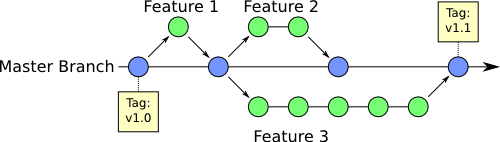
\includegraphics[width=0.8\textwidth]{featurebranch.png}
	\caption{Illustration of Feature Branch Workflow}
	\label{fig:featurebranch}
\end{figure}

When creating a new feature branch it normally only exist locally. If it is desirable to access it from several computers, or to share it with other users before it is done, it is possible to push it to the central repository (the origin). This, however, presupposes some good practices from the user: The branch should have a decent and globally understandable name, it should not exist on the server for too long, and the number of feature branches on the server should be kept somewhat small.

Finally, some revisions can be tagged with a version number, making it easier in publications to refer to a specific revision of the code. This should only be done with revisions on the master branch.

As a summary: feature branches can have many revisions allowing the developer to go back in case of mistakes, for backup, and for sharing code with other developers. The master branch is holy and only fully functional features should be merged into it.

If this section is unclear or more advice on Git is needed please refer to the ``Introduction to Git for \mnfysrppic{}'' available in \texttt{mn-fysrp-pic/docs/git.pdf} before making any changes to the repository.

\section{Setting up a Local Copy}
To access the repository and be able to make changes you need to set up a local copy. To get access you need an SSH key-pair (public and private keys). Unless you already have that you can run the following command\footnote{http://www.uio.no/tjenester/it/maskin/filer/versjonskontroll/git.html .}:

\begin{lstlisting}
	ssh-keygen -t rsa -b 4096
\end{lstlisting}

This generates the following files:
\begin{itemize}
	\item Private key: \lstinline$~/.ssh/id_rsa$
	\item Public key: \lstinline$~/.ssh/id_rsa.pub$
\end{itemize}
The private key is private (hence the name) and should under no circumstance be shared with others. It is what you use to access the remote server. The public key cannot be used to log on to a remote server but is rather used by the remote server(s) to verify that an log on attempt is in fact you (i.e. that you have the private key).

Rename a copy of your public key to \lstinline$<username>.pub$ and mail it to the repository administrator (sigvald.marholm@fys.uio.no) who has to accept your request and forward the message to the UiO IT department.

Next, configure your local git user like this:

\begin{lstlisting}
	git config --global user.name '<username>'
	git config --global user.email '<email>'
\end{lstlisting}
Go to the folder where you'd like your local copy (typically your home directory), and clone the central repository (origin) like this:

\begin{lstlisting}
	git clone gitolite@git.uio.no:mn-fysrp-pic
\end{lstlisting}
A new folder with the name \lstinline$mn-fysrp-pic$ will be created. This is your local working copy.

To get access from other computers you have to copy your private key to \lstinline$~/.ssh/id_rsa$ on those computers as well, and run the configuration and cloning steps there as well. You should typically have a local copy on your work station as well as on a supercomputer. Perhaps also on your private laptop if you wish.

\section{Folder Structure}
For working with the PIC code, your home folder should have the following sub-folders (unimportant details omitted):

\begin{itemize}
	\item \lstinline$mn-fysrp-pic$
	\begin{itemize}
		\item \lstinline$DiP3D$
		\begin{itemize}
			\item \lstinline$template$
			\item \lstinline$src$
			\item \lstinline$lib$
		\end{itemize}
		\item \lstinline$docs$
	\end{itemize}
	\item \lstinline$local_data$
	\begin{itemize}
		\item \lstinline$template$
		\item \lstinline$YYMMDD_<simulation description 1>$
		\item \lstinline$YYMMDD_<simulation description 2>$
		\item \lstinline$...$
	\end{itemize}
\end{itemize}

\lstinline$mn-fysrp-pic$ is the local working copy of the Git repository and is obtained by cloning the central repository as described in the previous section. \lstinline$mn-fysrp-pic/docs$ contain the documentation of the repository (this document) as well as auxiliary files used to create the documentation.

The source code for DiP3D is located at \lstinline$mn-fysrp-pic/DiP3D/src$. The primary task of the repository is to act as a Version Control System (VCS) for the code (.c-files) within this folder. The repository should not hold object (.o) files, compiled and linked executables, binaries or similar. VCSs like Git only needs to keep track of the lines changed in text files which makes them very efficient. Other files such as executables and object files carry no real information to the programmer and must be re-stored in entirety every time it changes (after each compilation). Many such files can make the repository heavy. It also clutters the repository with unnecessary changes each time someone recompiles the whole program, causing unnecessary Git conflicts.
The same is true for simulation files, which are incredibly large and not to be stored in the repository. There is also no reason to have version control on them; once a simulation is successfully run, and maybe even used in publications, it should be considered static. Simulations and their input files are also not, strictly speaking, part of the program, but rather something that changes from execution to execution.

Third party libraries shipped with the code are stored in \lstinline$mn-fysrp-pic/DiP3D/lib$.

The \lstinline$local_data$ folder is created as follows:

\begin{lstlisting}
	cd mn-fysrp-pic
	./setup_folders.sh
\end{lstlisting}

All the simulation-specific files are stored in sub-folders in \lstinline$local_data$ in order to separate it from the repository. Each simulation has exactly one sub-folder, which should be named \lstinline$YYMMDD_<simulation description>$ where YYMMDD is the date in reverse order. The sub-folders will contain the simulation results, as well as all the information necessary in order to make the numerical experiment reproducible: input files, job script, and information on exactly which Git revision of DiP3D was used to generate the result.

After simulation is done, the simulation data sub-folders should be copied to \lstinline$some_server.uio.no/path/to/DiP3D_data/$ (TBD: folder not created yet). This server is automatically backuped by the IT department.

The \lstinline$local_data/template$ folder contains example input files which serves as a starting point for making new simulation results. It is simply a copy of \lstinline$mn-fysrp-pic/DiP3D/template$. If for instance the format of the input files change, the template in the repository can be updated and \lstinline$setup_folders.sh$ can be run again to renew \lstinline$local_data/template$. All previously existing files in \lstinline$local_data/template$ will then be deleted, but all other files in \lstinline$local_data$ will persist.

\section{Running a Simulation}
Running a DiP3D simulation while keeping folders clean is easily done as described in this section.

First, you should checkout from Git the revision of DiP3D you'd like to use. Next, a new simulation data folder must be made. Here, we use the template as a starting point (a previously run simulation would also work):

\begin{lstlisting}
	cd local_data
	cp -r template 150611_test_simulation
	cd 150611_test_simulation
\end{lstlisting}
For the time being, the template contains the input files input.txt and sphere.txt which is edited according to the simulation in quest.

\subsection{Abel Supercomputer}
Next, to execute the job on Abel the job script \lstinline$start_abel$ is edited according to the users demands (with respect to resource usage and such) and executed:

\begin{lstlisting}
	sbatch start_abel
\end{lstlisting}

The job script copies all DiP3D source files and input files to Abel's scratch area before building the source and executing the simulation. This is the procedure recommended by USIT since the scratch area is faster. The simulation results are copied back to the data sub-folder after execution. This is true even if the program is terminated unexpectedly. The job scripts also generates a file called \lstinline$execinfo.txt$ which contains information about exactly which Git revision of DiP3D was used to produce the results, as fetched from Git itself. The file \lstinline$ompiinfo.txt$ contains the output of the bash command \lstinline$ompi_info$ showing information on versions of OpenMPI, compilers and miscellaneous. SLURM also writes its output file to this folder.

Abel will automatically delete the scratch folder including all object files and executables. Neither the repository nor the \lstinline$local_data$ folder will be cluttered with these files. Finally, you should take a copy of the data sub-folder to \lstinline$some_server.uio.no/path/to/DiP3D_data/$ (TBD: folder not created yet)

\subsection{Desktop Computer}
On a plain desktop computer the code can be run without MPI like this:

\begin{lstlisting}
	./start_plain.sh
\end{lstlisting}

\lstinline$start_plain.sh$ creates a scratch folder within the data folder which acts the same way as scratch on Abel. This folder is deleted if the execution script is successfully run. The information files are generated also in this case.


\end{document}
